Resultatet baseras på svaren till frågorna i bilaga \ref{apdx:fragor} givna i intervju med Daniel Johansson på MacGregor. %\cite{daniel}.

%
%   INTERVJU
%

\subsection{Intervju}
% Vad används?
På MacGregor är den vanligaste produktkalkylen en ABC-kalkyl och den är ett tungt vägande styrmedel givet dess precision.
Utöver ABC-kalkyl nämndes även direkt kostnadspåslag.
Detta var dock mycket mer ovanligt då den inte har samma precision.

% Varför?
Anledningen att ABC-kalkylen tillämpats trots sin inneboende komplexitet är att den ger bäst uppskattning.
MacGregor menar på att den ger en kontroll över kostnader samt ett effektivt beslutsunderlag för vinstdrivandet inom företaget som andra modeller ej ger.
Företaget handskas ofta med flera olika valutor, vilket fort ställer till med problem då alltför enkla modeller används.
Detta är något man kan handera med hjälp av ABC-kalkylen.
Man använder en detaljerad ABC-kalkyl med totalt 24 aktiviteter.
Detta för att man lätt ska kunna se var man har besparingsmöjligheter.
Istället för att utföra intervjuer med personal så har man ett affärssystem där tider rapporteras.
Detta gör att man sparar mycket tid och får fram sin ABC-kalkyl mycket smidigare.
Det ger även en kontinuerlig bild av alla aktiviteter och hur mycket tid som läggs på dessa.

% Situationer?
Denna typ av kalkyl används på samtliga offerter.
Så fort en kund kommer och frågar om en produkt så utförs en beräkning.
Det görs även för utvecklingsprojekt.
Till exempel tittar man på möjligheten till att göra förändringar som kan leda till besparingar.
Ett tredje område där denna kalkyl används är investering.

% Expempel på produktkalkyl
Ett exempel på de olika kalkylposter som ingår i deras ABC-kalkyl kan ses i figur \ref{fig:abc}.
\begin{figure}[ht]
    \centering
    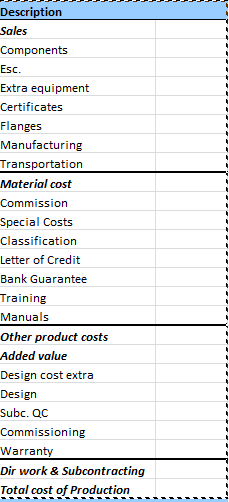
\includegraphics[scale=.6]{img/abc.png}
    \caption{Exempel på kalkylposter från MacGregor}
    \label{fig:abc}
\end{figure}
Det påpekas att detta är en väldigt generell modell.

% För- och efterkalkyl?
Det görs både för- och efterkalkyler då alla produkter är speciella.
Daniel säger att ''Du gissar alltid till viss mån och och du vill alltid veta vad resultatet är." \cite{daniel}.
Man vill speciellt kunna ha koll på alla valutaeffekter.

% Hur ser skillnaderna ut?
MacGregor har lyckats få en mycket bra precision med hjälp av denna metod.
Enligt företaget anses en avvikelse på 2\% vara mycket stor.
Denna noggrannhet har uppnåtts först under de senaste 5 åren.

% Hur ser det ut i de olika situationerna?
Kalkylen kan se lite olika ut beroende på situationen där den används.
Då en offert görs används en mer generell modell.
Då en ny produkt ska tas fram behövs dock en mer detaljerad bild.
Det tillkommer då poster som till expempel projektledning, säljare, och marknadsföring.
Man behöver även se över eventuella utbildningar och titta på den interna produktionskostnaden.
Det krävs mycket mer detaljer för att det ska gå att kunna följa upp med en efterkalkyl.
I intervjuven nämns även att det kan bli speciellt för just MacGregor.
Företaget arbetar med marina produkter som har stora krav.
Användandet av flera olika valutor och dess påverkan nämns även igen.
Detta gör att varje kalkyl blir unik.

% Vem/vilka uträttar?
% Hur ofta?
Dessa kalkyler upprättas av Daniel själv, men även utesäljare har verktyg för att med enkla medel kunna utföra kalkyler. 
Tillverkningsunderlag finns tabulerat så de väljer vilken produkt de ska sälja så ger programmet det som behövs, men det är Daniel som sammanställer all data.
Dessa kalkyler utförs dagligen och man har tre dedikerade säljare som inte jobbar med något annat än att utföra dessa kalkyler.

% Datakällor?
För att kunna utfärda dessa kalkyler används en del datakällor så som efterkalkylsdata, all känd offertdata, specialkomonenter till störst del, men även teknisk data då tekniken måste sitta ihop med produkten och alla ritningar.
Det kan vara svårt att göra kalkylerna förrän i slutskedet av produkten då all data finns att tillgå.  

% Vilka använder kalkylerna?
Först och främst är det säljarna som behöver kalkylerna för att kunna sätta ett pris på produkten.
Hela ekonomiavdelningen är dock starkt beroende på kalkylerna då man till exempel gör månadsuppföljningar.
Även de personer som har hand om, och som följer upp, kontrakt behöver ta del av dem.
I kalkylen finns det beskrivet hur mycket tid och pengar som planerats att användas.
På grund av detta så behöver, på ett eller annat sätt, alla som arbetar med produkten ha tillgång till kalkylen.

% Är man nöjd med hur den utförs?
Generellt sett är man väldigt nöjd med hur produktkalkyleringen utförs på företaget.
Säljarna tycker självklart att det alltid är för dyrt.
Det finns stor precision i hur systemet fungerar.
Det är lätt för slutanvändarna att använda kalkylerna.
Daniel menar dock att han själv får jobba ganska hårt för att det ska fungera så smidigt som det gör.

% Senaste ändringar som gjorts?
En av de senaste ändringar som gjorts inom företaget är ett byte av koncernvaluta.
Att använda flera olika valutor leder ofta till knepiga situationer.
Det föregående system som MacGregor använde kunde ej hantera flertalet valutor på ett bra sätt.
Detta är något som är fixat.

Affärssystemet som används på MacGregor låter alla anställda rapportera timmar spenderat på en viss aktivitet.
På grund av detta får företaget en kontinuerlig bild av vilka aktiviteter som utförs.
Detta ger dem en stark bas för deras ABC-kalkyl.

% Planerade förändringar
Just nu planeras inga övergripande förändringar i företagets produktkalkyler. Företaget uppdaterar kontinuerligt alla kalkyler men något övergripande eller omvälvande sades det inget om.

% Egna frågor, eg strul vid olika valutor
Att arbeta med flera olika valutor var något som återkom ofta i intervjuven med MacGregor.
Det kan lätt bli väldigt krångligt, och Daniel rekommenderar ej andra företag att arbeta med mer än en valuta om det inte behövs.
När en kalkyl upprättas har en valuta ett visst värde enligt kursen.
Med tiden förändras dock denna valutakurs.
MacGregor gav oss ett exempel på hur detta kan ställa till problem.
Säg att företaget budgeterar 400 timmar till en designer med en viss valutakurs.
Med tiden förändras detta.
Efter 300 timmar så är alla pengar slut, även om designern tycker sig ha 100 timmar kvar att arbeta med.
Detta kan givetvis svänga åt andra hållet också, då man får pengar över även när man använt all planerad arbetstid.

%
%   JÄMFÖRELSE
%

\subsection{Jämförelse med teori}

MacGregor använder sig av ett dynamiskt antal aktiviteter, men ofta av storleksordningen 20-30 stycken, vilket är mer än vad som framställts som nödvändigt i litteraturen ''Den nya ekonomistyrningen" \cite{dne} samt vad som sagts på föreläsningar på Luleå Tekniska Universitetet.
Argumentet som förs fram för att styrka ett lågt antal aktiviter brukar vara att det blir en hög komplexitet och därmed dyrt.
MacGregor verkar däremot inte ha några problem med det, utav vill ha den för att vinna precision vilket i sin tur blir mer lönsamt trots den ökade kalkylkostnaden.

% Intervju minimering m teknik
MacGregor använder sig av tekniska lösningar för att minimera mängden tid ekonomen behöver lägga på att lista ut hur mycket tid varje aktivitet egentligen använder.
\cite{dne} skriver att uppstartskostnaden för en ABC-kalkyl är stor samt att underhållskostnaden är stor.
Med hjälp av dessa tekniska lösningar har MacGregor därmed lyckats minska underhållskostnaden för kalkylen.

% Automatisering
Vidare använder ekonomerna på MacGregor programmering och andra automatiationsverktyg för att förenkla uppställningen och underhållet av kalkylen.
Detta minskar omkostnaderna för att ha en ABC-kalkul rullande på företaget.
Det ska dock noteras att dom är 3 heltidsanställda som inte gör annat än att räkna på dessa kalkyler.

% Val av kalkylsort
Eftersom ABC-kalkylen är mer precis än till expempel påläggskalkylen så använder MacGregor denna då precisionen leder till mycket större vinster än de möjliga besparingarna på att använda en annan kalkyl.
Dom får helt enkelt en bättre bild av vad pengarna går till.

% Totalt stämmer klassrummet bra överens med svaren fr inteervjjun, B0rtsrtt från detaljnivån.
Totalt sett är det mesta som förväntat när man jämför MacGregors implementation av kalkylen med teorin.
Tekniken har underlättat för ekonomerna och därmed minskat omkostnaderna samt ökat precisionen.
Detta undertrycks inte i litteraturen eller på föreläsningarna.